\documentclass[11pt]{article}

%------------------------- Packages -------------------------
\usepackage[margin=1in]{geometry}
\usepackage{amsmath, amssymb}
\usepackage{graphicx}
\usepackage{listings}
\usepackage[hidelinks]{hyperref}
\usepackage{enumitem}
\usepackage{indentfirst}
\usepackage{titling}

% Figures are resolved from results/figures/ (this file lives in results/reports/).
\graphicspath{{../figures/}}

%------------------------- Paragraph indentation -------------------------
\setlength{\parindent}{2em}
\setlength{\parskip}{0pt plus 1pt}
\setlength{\droptitle}{-1.75cm}

%------------------------- Code style -------------------------
\lstset{
    basicstyle=\ttfamily\small,
    breaklines=true,
    frame=single
}

\title{\textbf{Lab2 Report}}
\author{}
\date{}

\begin{document}
\maketitle

\section*{Task 1}
The results of the latency-throughput curves under different traffic patterns are shown in Figure~\ref{fig:task1}.

At low load the latency is almost entirely zero-load network latency, which is
determined by the hop count, so the low-load latency ordering follows the
average hop count exactly: neighbor ($\approx 1.75$ hops, $\approx 8.5$
cycles), tornado ($\approx 3.75$ hops, $\approx 12.5$ cycles), shuffle
($\approx 4.0$ hops, $\approx 13.0$ cycles), uniform random ($\approx 5.27$
hops, $\approx 15.6$ cycles) and transpose ($\approx 5.31$ hops,
$\approx 15.6$ cycles).

As the load increases, the four non-neighbor patterns all eventually saturate,
and their behavior diverges according to the spatial distribution of traffic.
Uniform random spreads packets evenly with no hotspots, so it saturates the
latest and reaches the highest throughput among the four ($\approx 0.34$
flits/cycle/node); transpose, whose (row, column) $\to$ (column, row) mapping
concentrates traffic near the diagonal, saturates the earliest and with the
lowest throughput ($\approx 0.27$); tornado ($\approx 0.27$) and shuffle
($\approx 0.29$) lie in between. Neighbor, whose packets travel only about one
hop on average, never saturates within the tested range.

Interestingly, at rate $0.5$ transpose has the lowest latency among the four
saturated patterns ($\approx 937$ cycles, versus $\approx 1208$ for uniform
random, $\approx 1440$ for shuffle and $\approx 1499$ for tornado), even
though it saturates the earliest. The reason is that, once saturated, the
completed packets are increasingly dominated by the short-hop ones near the
diagonal: long-hop packets suffer the most contention and are starved, so the
average hop count of completed packets declines (from about $5.3$ to $2.7$ for
transpose) and drags the average latency down. For the other patterns the
average hop count stays roughly constant over the tested range.

\begin{figure}[htbp]
    \centering
    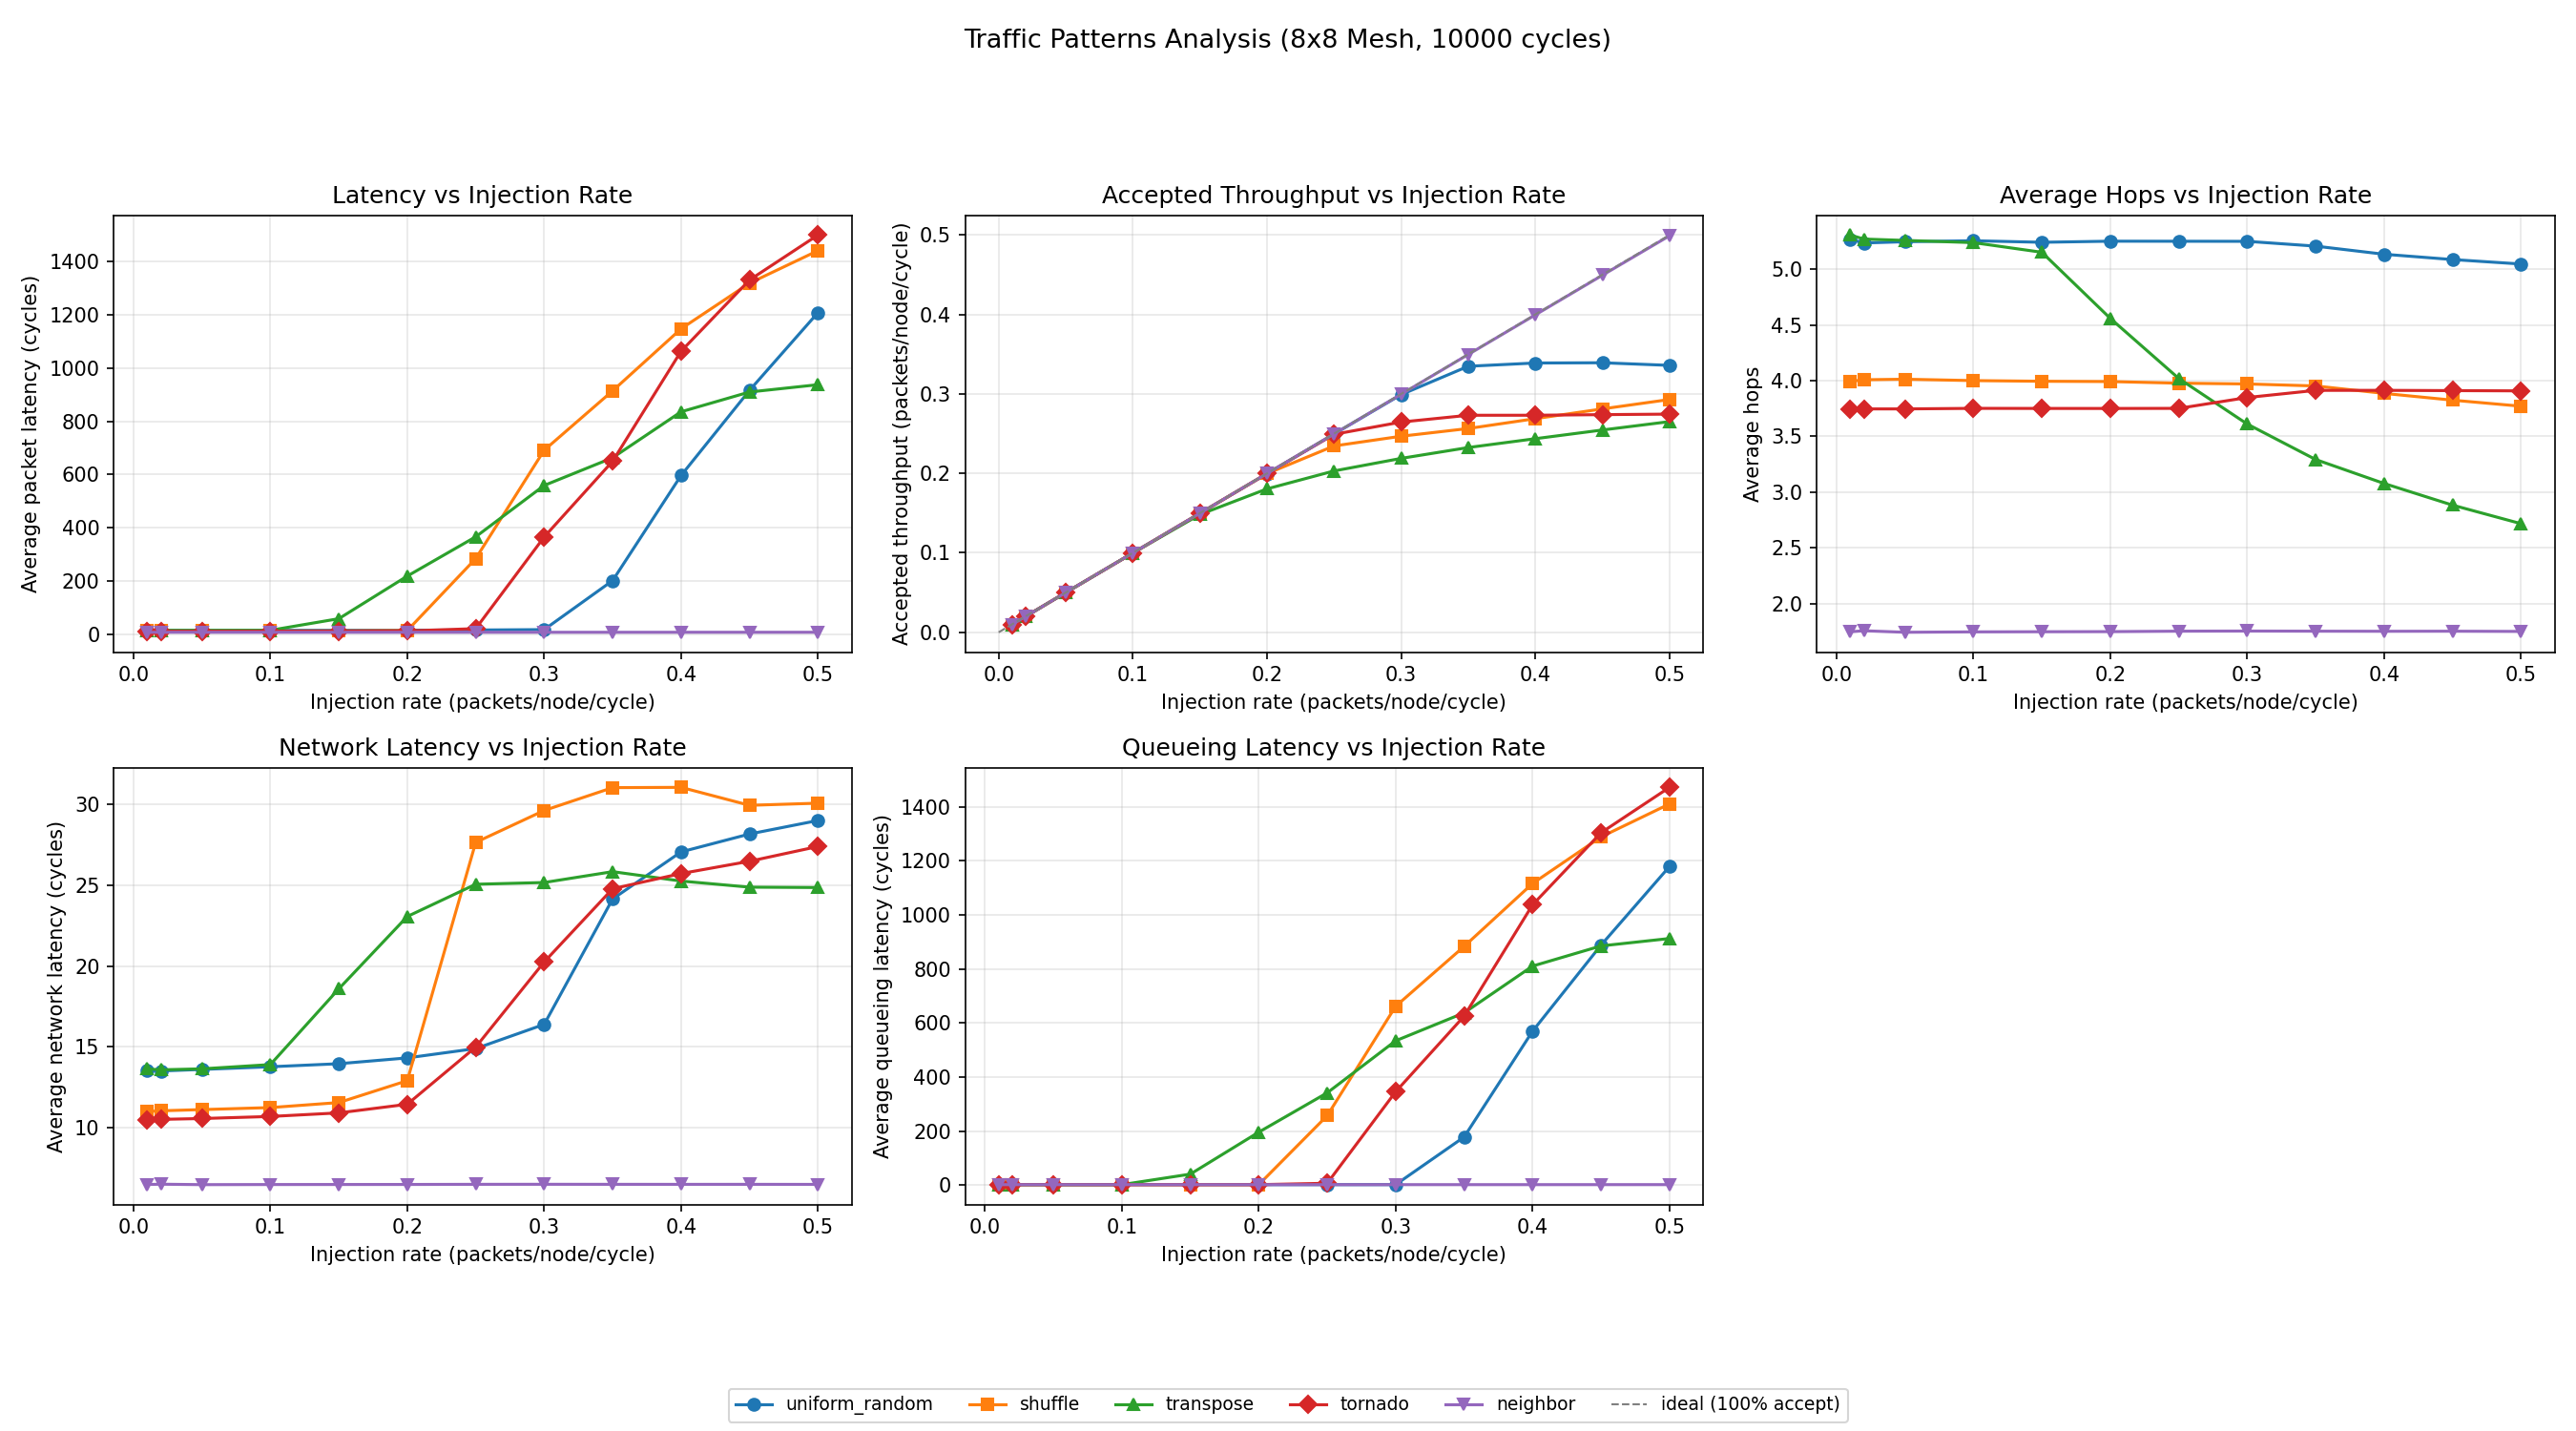
\includegraphics[width=0.9\textwidth]{lab2_task1_analysis.png}
    \caption{Latency and throughput versus injection rate for the five traffic
    patterns on the 8$\times$8 Mesh.}
    \label{fig:task1}
\end{figure}

\section*{Task 2}
All sweeps use uniform random traffic on the 8$\times$8 Mesh as the baseline
(vcs-per-vnet = 4, router latency = 1, link width = 128 bits) and change one
parameter at a time.

The decline of the average hop count with increasing load indicates that, once
the network saturates, only packets with shorter routing paths are successfully
delivered, whereas packets with longer paths are starved and fail to complete
within the simulation window.

\textbf{VCs per vnet.} (Figure~\ref{fig:task2_vcs}) The number of VCs does not change the low-load latency,
but it clearly shifts the saturation behavior: with more VCs, saturation occurs
later, the saturation throughput is higher, the saturated latency is lower, and
the clear decline of the average hop count is delayed, because more VCs reduce
head-of-line blocking. The saturation throughput grows with the VC count: a
single VC saturates almost immediately ($\approx 0.07$), 2 VCs reach
$\approx 0.16$, 4 VCs reach $\approx 0.34$, and 8 VCs reach $\approx 0.39$.

\textbf{Router latency.} (Figure~\ref{fig:task2_router}) Router latency mainly raises the zero-load latency of
the entire curve, since each extra pipeline stage adds one cycle per hop. It also
affects saturation: as the latency decreases, saturation occurs later, the
saturation throughput is higher ($\approx 0.34$ for latency 1, $\approx 0.29$
for latency 2, and $\approx 0.21$ for latency 4), the saturated latency is
lower, and the clear decline of the average hop count is delayed. With 4
pipeline stages the network saturates noticeably earlier because each hop
occupies the link longer.

\textbf{Link width.} (Figure~\ref{fig:task2_linkwidth}) In Garnet the flit size scales with the link width
(\texttt{ni\_flit\_size = link\_width\_bits/8}). Widening the link from 32 to
64 bits brings a clear improvement: at 32 bits the 8-byte control packet is
split into two 4-byte flits, which doubles the serialization cost, so the
network saturates earlier and at a lower throughput ($\approx 0.15$). From 64
bits onward the packet already fits in a single flit, so the 64, 128, and
256-bit curves overlap exactly and reach the same throughput ($\approx 0.34$)
as the baseline, and widening the link has no further effect.

\begin{figure}[htbp]
    \centering
    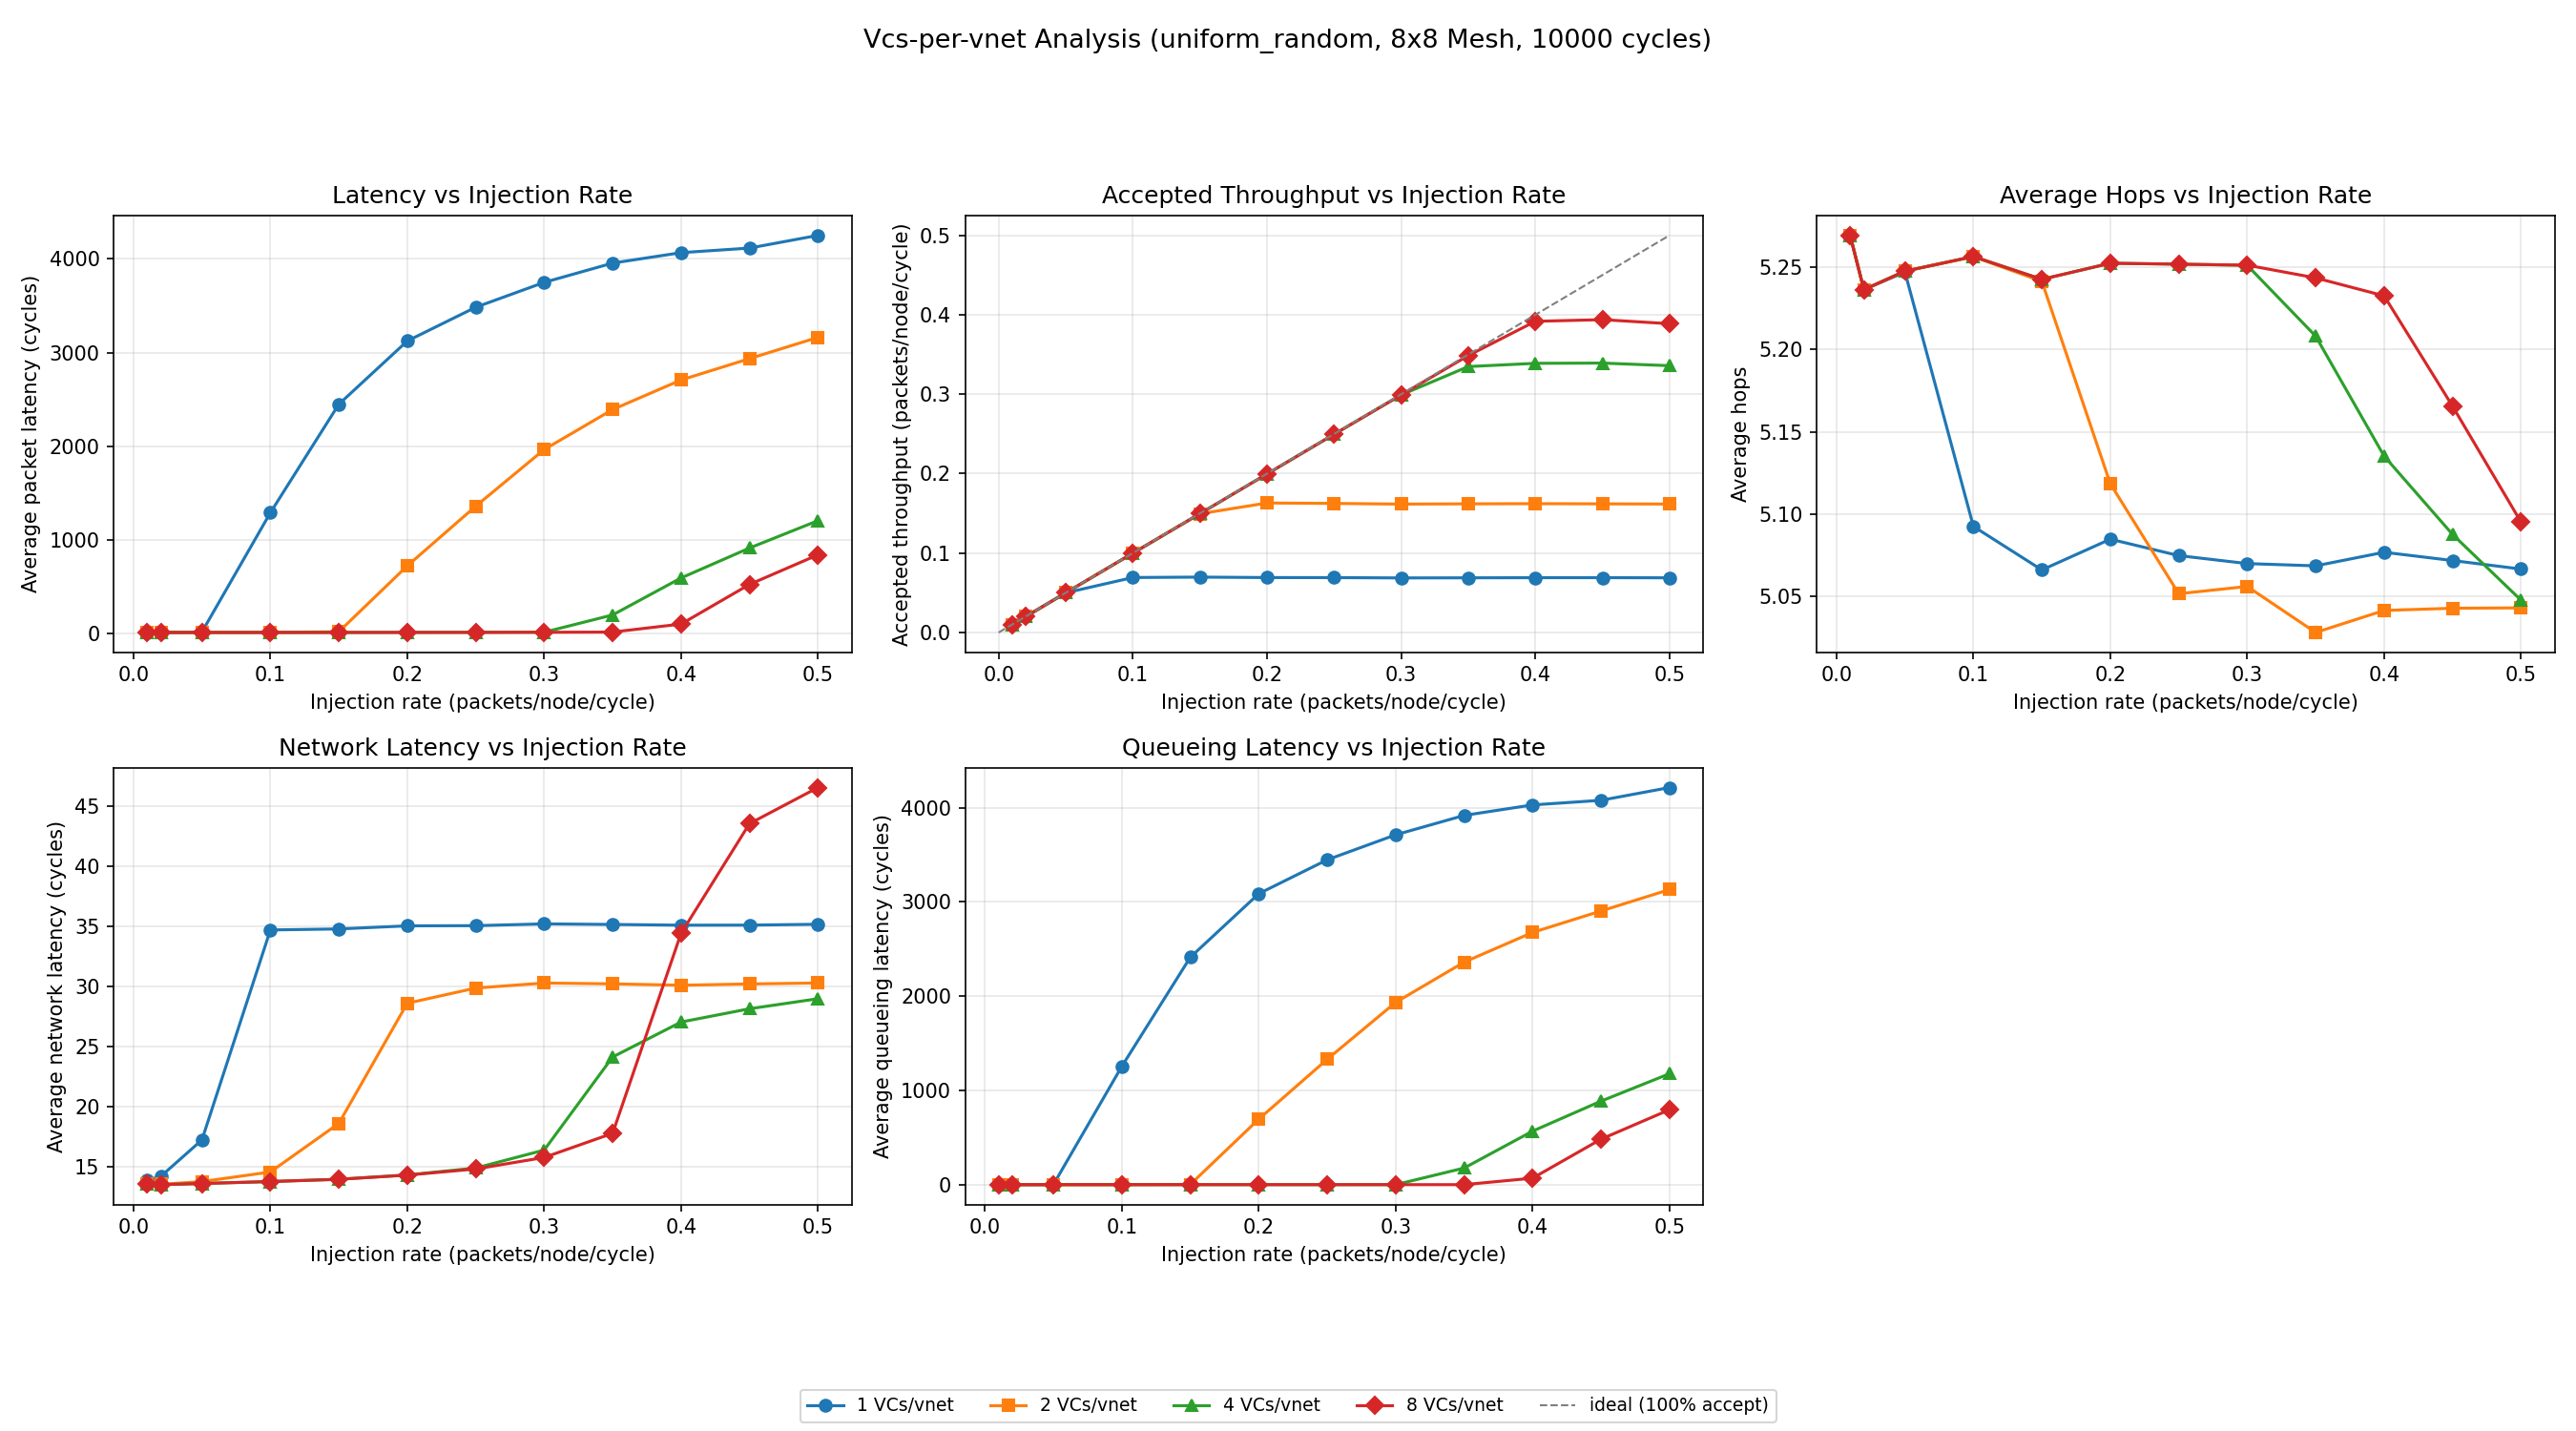
\includegraphics[width=0.9\textwidth]{lab2_task2_vcs_analysis.png}
    \caption{Latency and throughput versus injection rate under different VCs
    per vnet (uniform random traffic).}
    \label{fig:task2_vcs}
\end{figure}
\begin{figure}[htbp]
    \centering
    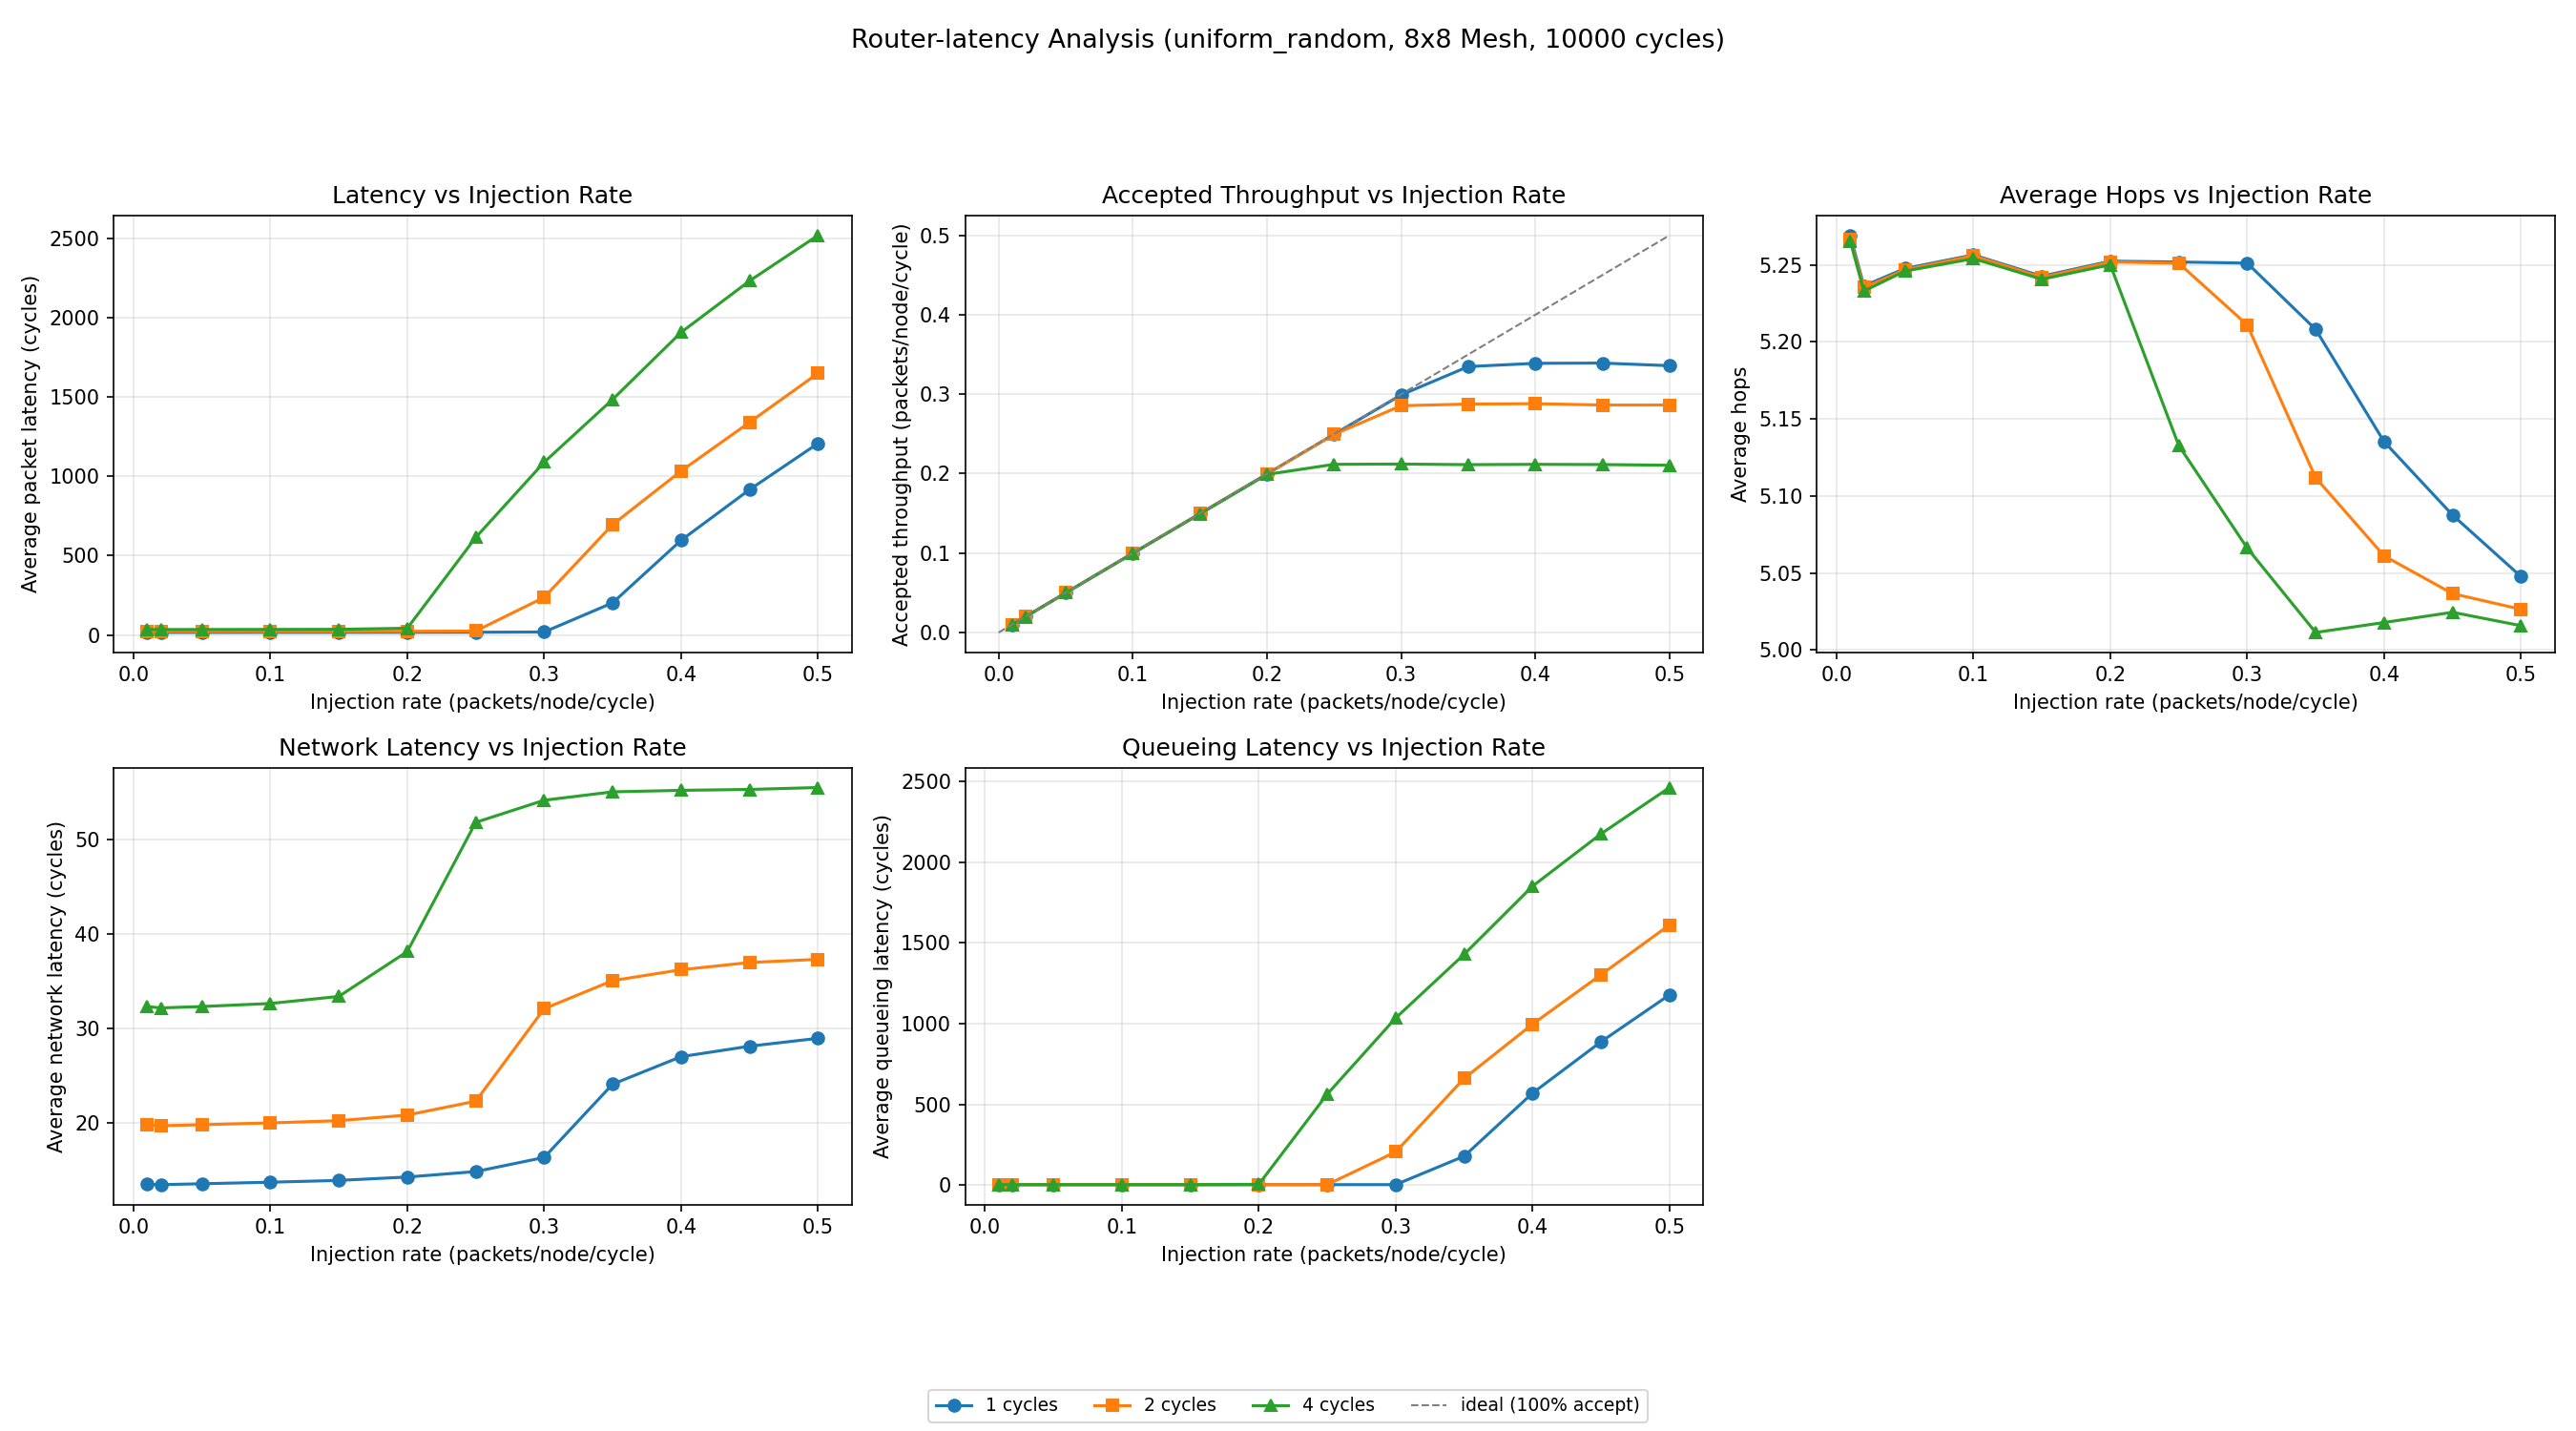
\includegraphics[width=0.9\textwidth]{lab2_task2_router_analysis.png}
    \caption{Latency and throughput versus injection rate under different
    router latencies (uniform random traffic).}
    \label{fig:task2_router}
\end{figure}
\begin{figure}[htbp]
    \centering
    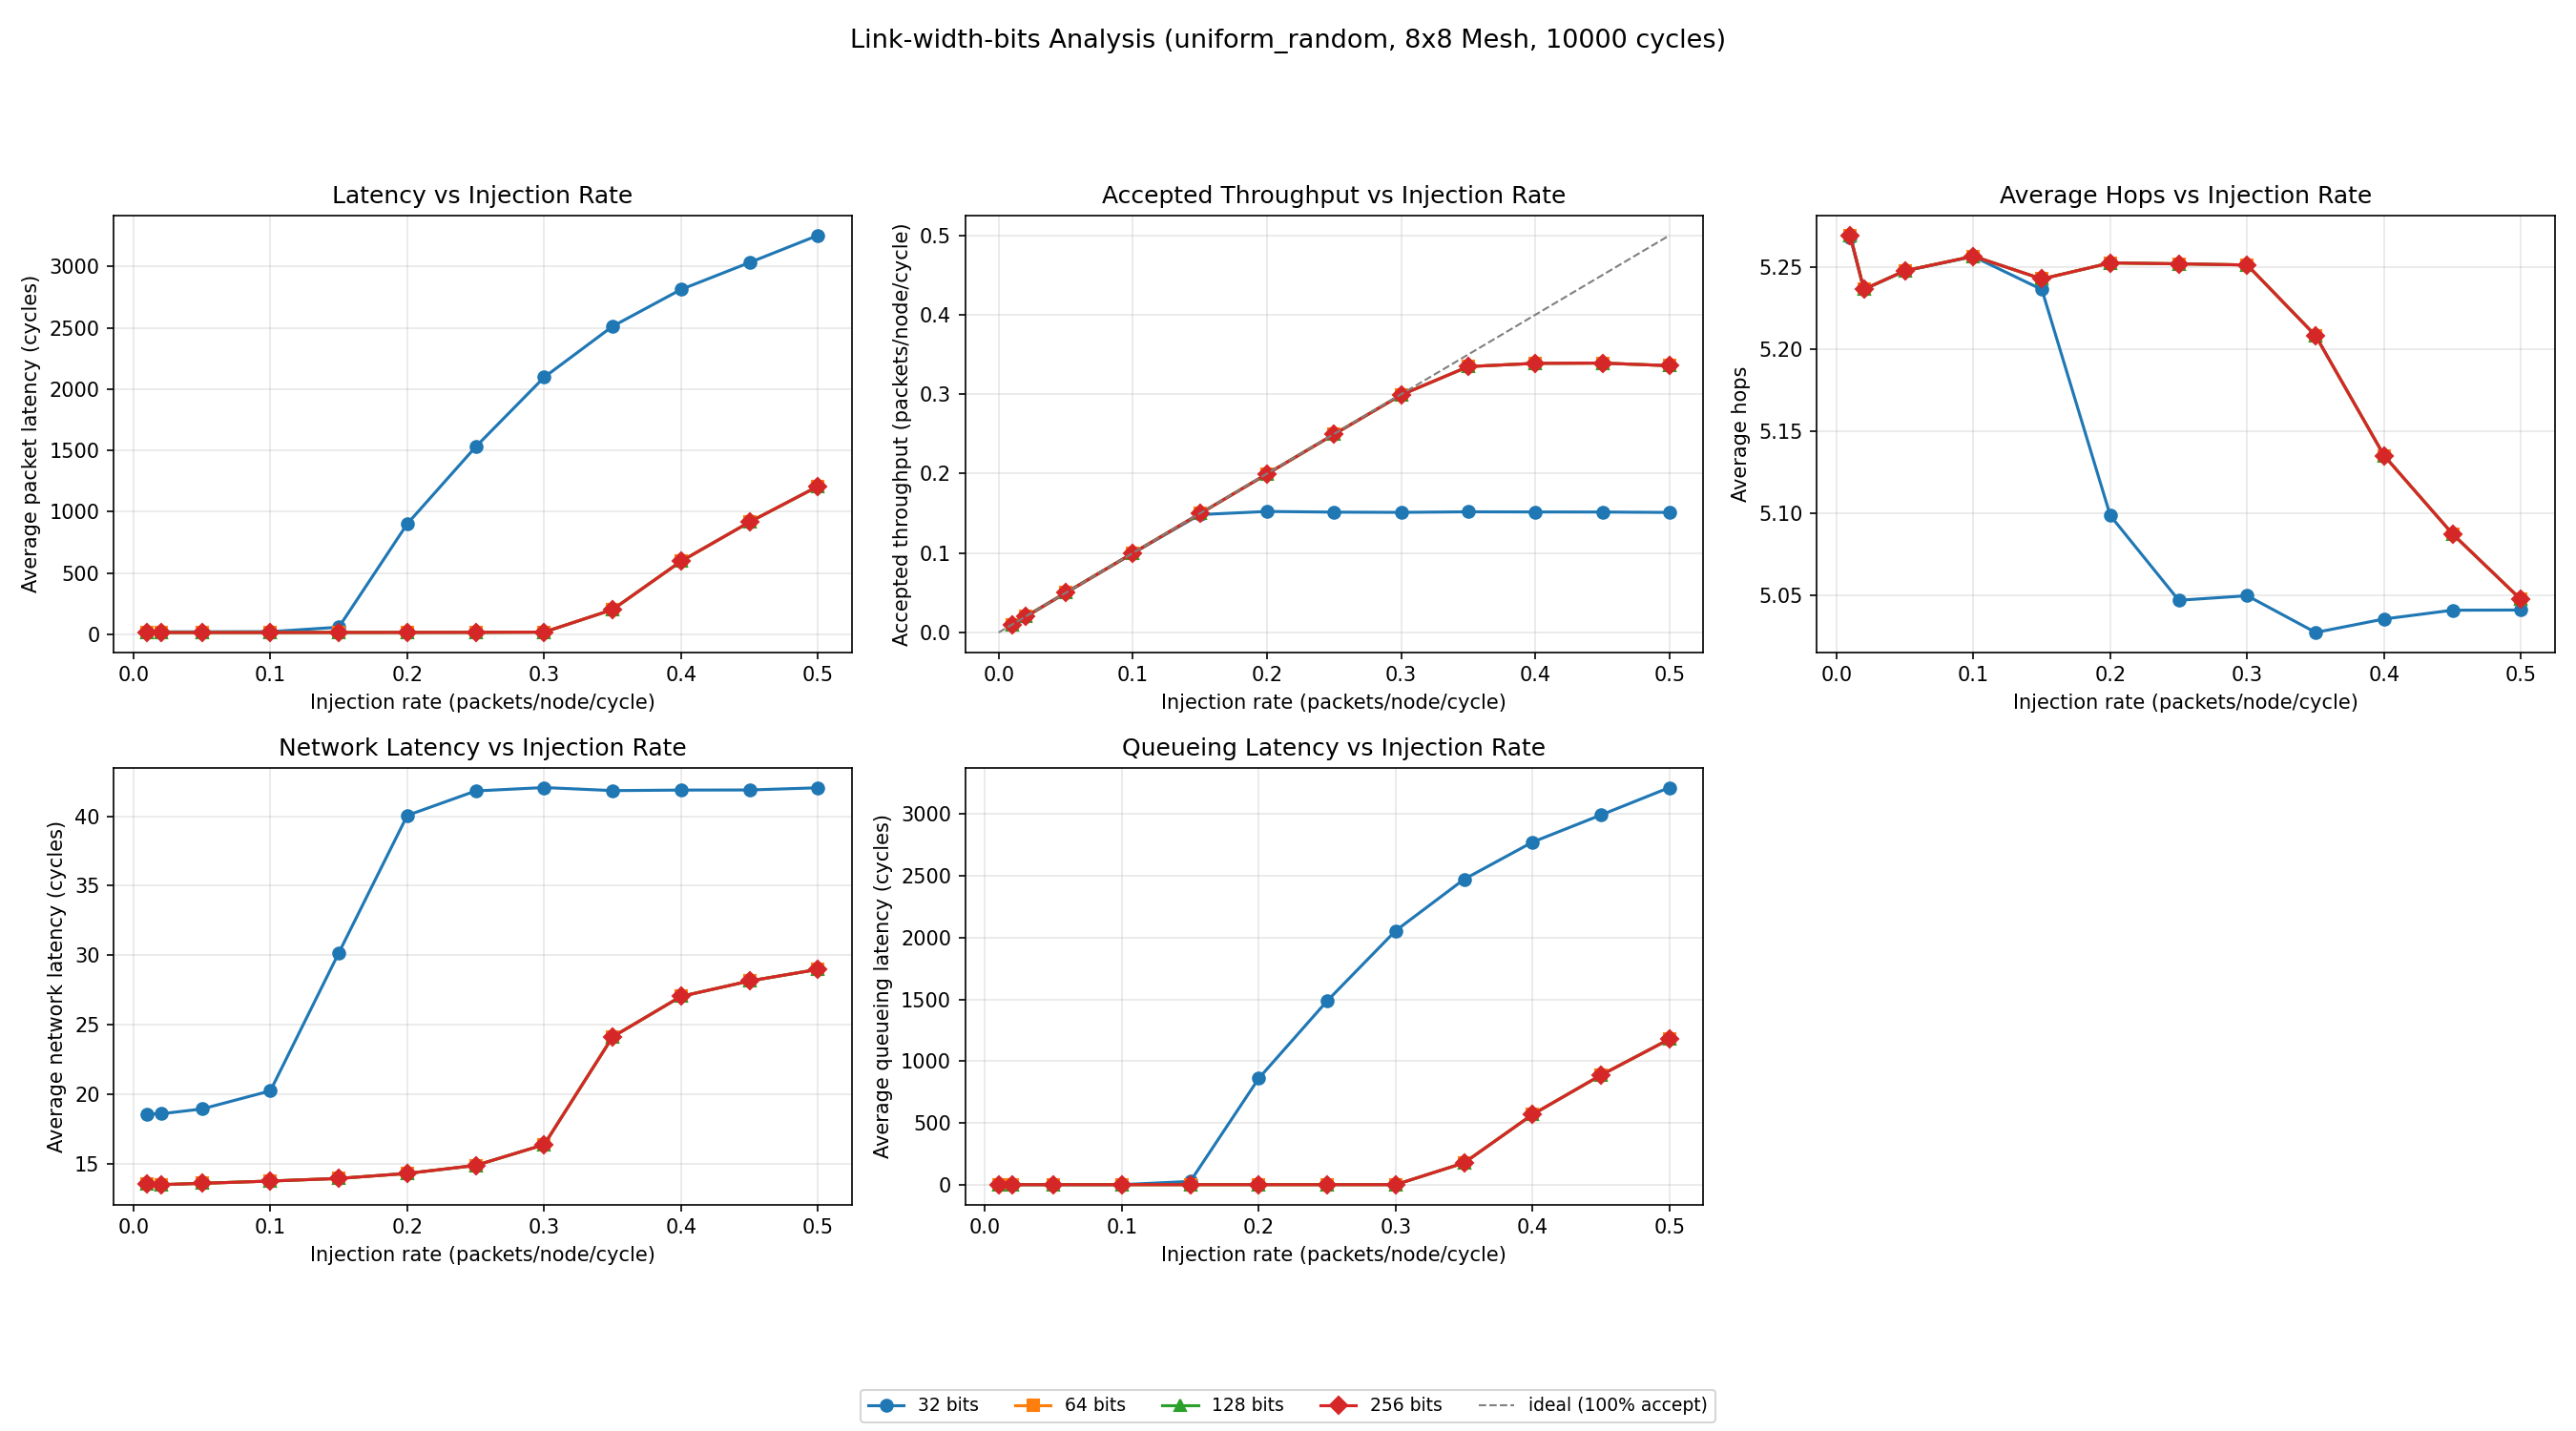
\includegraphics[width=0.9\textwidth]{lab2_task2_linkwidth_analysis.png}
    \caption{Latency and throughput versus injection rate under different link
    widths (uniform random traffic).}
    \label{fig:task2_linkwidth}
\end{figure}

\section*{Task 3}
\subsection*{Q1}
What are the components of network latency? Which component is dominant/bottleneck (for different traffic patterns/loads/linkwidths)?\\

Packet latency can be decomposed into network latency plus queueing latency. Under the neighbor traffic pattern, queueing latency stays negligible even as the load increases (the injection rate is at most $0.5$ in our experiments), so the total packet latency remains close to its low-load value. Under all other traffic patterns and link widths, queueing latency dominates the total latency at heavy load (the injection-rate threshold is around $0.2$, and it varies with the traffic pattern and link width), whereas at low load the latency is almost entirely network latency. (Here, network latency refers to the latency of a packet traversing the links: under zero load it equals $\text{hops} \times (\text{router latency} + \text{link latency}) + \text{serialization}$, and at heavy load it additionally includes in-network contention, e.g., waiting for VC/switch allocation or credits.)

\subsection*{Q2}
What is the depth of input buffer and the default flow-control?\\

The input buffer depth depends on the vnet type: $4$ flits for data VCs and $1$ flit for control VCs, and the default flow control is credit-based.

\end{document}
